\section{Experimental Evaluation}
\label{sec::experimental-evaluation}

\subsection{BP-MDS Execution and Evaluation}

\begin{figure*}[t]
    \centering
    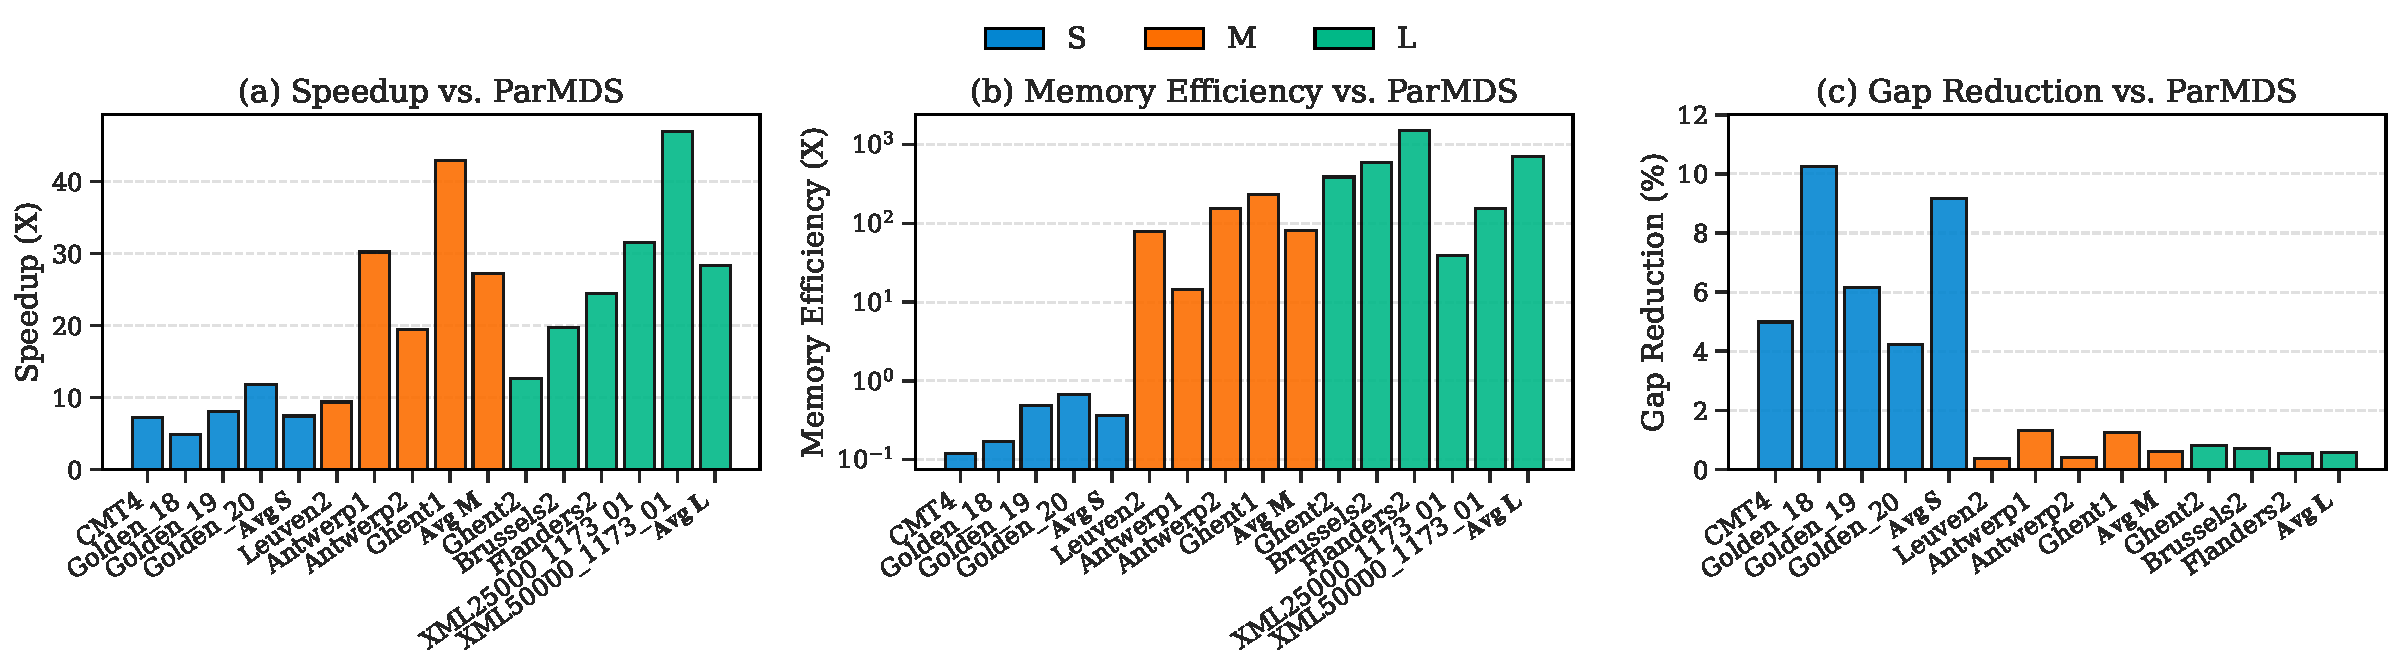
\includegraphics[width=\linewidth]{sections/results/parMDS.pdf}
    \caption{BP-MDS vs.\ ParMDS performance}
    \label{fig:parMDS_comparison_grid1}
\end{figure*}

\begin{figure*}[ht]
    \centering
    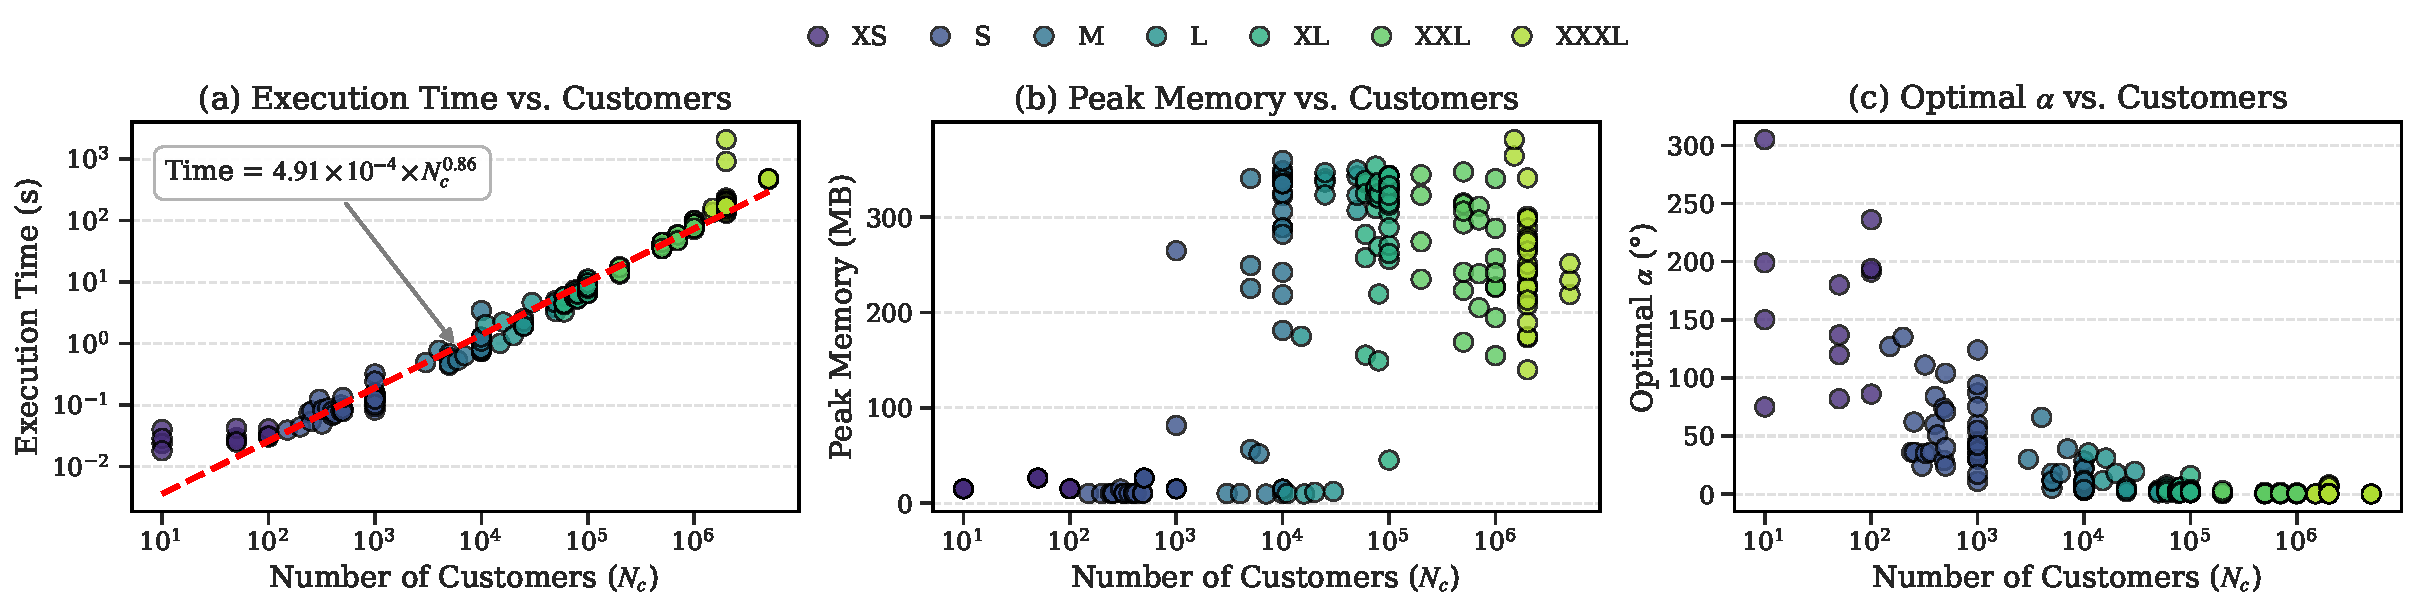
\includegraphics[width=\linewidth]{sections/results/node_Results.pdf}
    \caption{Scalability of BP-MDS: execution time, peak memory and $\alpha$ vs.\ number of customers}
    \label{fig:scalability_grid}
\end{figure*}

To facilitate consistent and scale-aware comparisons, we group datasets into size-based categories based on the number of customers:
XS (1 to 100), S (101 to $10^3$), M ($10^3\!+\!1$ to $10^4$), 
L ($10^4\!+\!1$ to $5\times10^4$), 
XL ($5\times10^4\!+\!1$ to $10^5$), 
XXL ($10^5\!+\!1$ to $10^6$), and 
XXXL ($10^6\!+\!1$ to $10^7$).
Metrics are reported within each category to avoid scale-induced bias in aggregated results. For instance, aggregating results across instances such as \texttt{Golden\_10} (324 nodes) and \texttt{XML\_500000\_3126\_01} (500{,}001 nodes) would otherwise bias the evaluation toward larger instances. All results are averaged over five runs to reduce variance and ensure stability. To reduce RSS overhead from per-thread stack allocation, we set \texttt{OMP\_STACKSIZE}=256KB, which we found sufficient empirically, as BP-MDS uses iterative implementations, heap-allocates its core data structures, and requires minimal stack space. Larger per-thread stacks (4--8 MB) would otherwise increase memory overhead under nested parallelism.

\textbf{Experimental Setup:} All experiments were conducted on a dual-socket Intel Xeon Gold 6248 system with 20 physical cores (40 logical cores) running at 2.50\,GHz, 27.5\,MB of L3 cache, and 192\,GB of RAM. The system runs Red Hat Enterprise Linux 7.6 (64-bit). BP-MDS and all baseline methods were compiled using GCC 9.2.0 with the \texttt{-std=c++17}, \texttt{-O3}, and \texttt{-fopenmp} compiler flags.


\textbf{Input Instances:} We evaluate BP-MDS on 310 CVRP instances\footnote{\label{fn:github}160 synthetic benchmark instances and the optimal BP-MDS partition angle ($\alpha$) for all 310 instances are available in our \href{https://github.com/CodeCraftsmanSandeep/BP-MDS}{GitHub repository}} comprising 130 benchmark instances from CVRPLIB~\cite{Uchoa_CVRPLIB,CVRPLIB}, including X (1--101), Golden (9--20), Antwerp (1--2), Brussels (1--2), Flanders (1--2), Ghent (1--2), Leuven (1--2), CMT5, E-n76-k (10,14), E-n101-k (8,14), F-n135-k7, P-n101-k4, and tai385. To assess scalability, we further include 20 large-scale FILO2 instances~\cite{FILO2} and 160 synthetic (\texttt{XML}-prefixed) instances generated using the CVRPLIB instance generator, covering seven problem scales (XS--XXXL) ranging from $10$ to $5\times10^{6}$ customers. Solution quality ($\mathrm{Gap}=(\mathrm{Cost}-\mathrm{BKS})/\mathrm{BKS}\times 100\%$) is evaluated against the Best-Known Solutions (BKS) reported by CVRPLIB for the 130 benchmark instances and by Accorsi and Vigo~\cite{FILO2} for the 20 FILO2 instances.


Table~\ref{tab:bpmds_per_instance_results} presents per-instance performance, demonstrating scalability to instances with up to 5 million nodes, which are solved within 8 minutes. Table~\ref{tab:avg_metrics_single} summarizes aggregated results across size categories, yielding an overall geometric mean optimality gap of 8.51\%. The 130 CVRPLIB instances achieve a geometric mean gap of 9.67\%\footnote{Reported optimality gaps are computed using the CVRPLIB BKS values available at the time of experimentation.}, while the 20 FILO2 instances achieve a geometric mean gap of 1.27\%. The lower gap on FILO2 is expected, as its Best-Known Solutions (BKS) are taken from the original benchmark, whereas CVRPLIB BKS have been progressively improved through extensive community contributions. To evaluate relative performance, we compare against ParMDS~\cite{Muniasamy_VRP} and the Hybrid Genetic Search (HGS) of Vidal~\cite{vidal2022hybrid}, two state-of-the-art baselines.

\begin{table}[htbp]
\caption{Class-wise aggregated performance of BP-MDS}
\centering
\small
\begin{tabular}{l r r r r r r r r}
\toprule
\multirow{2.5}{*}{\textbf{Size}} & 
\multicolumn{2}{c}{\makecell[c]{\textbf{Avg. Time} \\ \textbf{(s)}}} & 
\multicolumn{2}{c}{\makecell[c]{\textbf{Avg. Mem.} \\ \textbf{(MB)}}} & 
\multicolumn{2}{c}{\makecell[c]{\textbf{Arith. Mean} \\ \textbf{Gap (\%)}}} & 
\multicolumn{2}{c}{\makecell[c]{\textbf{Geo Mean} \\ \textbf{Gap (\%)}}} \\
\cmidrule(lr){2-3} \cmidrule(lr){4-5} \cmidrule(lr){6-7} \cmidrule(lr){8-9}
& \textbf{(a)} & \textbf{(b)} & \textbf{(a)} & \textbf{(b)} & \textbf{(a)} & \textbf{(b)} & \textbf{(a)} & \textbf{(b)} \\
\midrule
XS  & 0.03   & 0.03 & 4.66  & 4.66 & 8.75 & 8.75 & 8.74 & 8.74 \\
S   & 0.09   & 0.09 & 5.35  & 5.35 & 9.77 & 9.77 & 9.70 & 9.70 \\
M   & 1.84   & 1.84 & 17.01 & 17.01 & 9.77 & 9.77 & 9.73 & 9.73 \\
L   & 4.19   & 3.82 & 45.31 & 36.59 & 10.32 & 7.96 & 10.28 & 7.87 \\
XL  & --  & 14.52 & -- & 34.24 & -- & 2.11 & -- & 2.11 \\
XXL & -- & 171.11 & -- & 84.25 & -- & 1.13 & -- & 1.13 \\
\bottomrule
\multicolumn{9}{l}{\footnotesize (a) CVRPLIB 130 instances;  (b) CVRPLIB + FILO2 instances (130+20) instances}
\end{tabular}

\label{tab:avg_metrics_single}
\end{table}

\subsubsection{Comparison Against ParMDS}

We identify a discrepancy in ParMDS: the effective exploration parameter $\rho$ deviates by $\sim\!20\times$ from the reported value. For fairness, we set $\rho$ to the intended value; all reported ParMDS results use this corrected configuration. Fig.~\ref{fig:parMDS_comparison_grid1} compares the performance of BP-MDS against ParMDS. ParMDS exhibits a fundamental scalability limitation: it exhausts system memory beyond $\approx 5 \times 10^{4}$ nodes due to explicit materialization of the complete graph. In contrast, BP-MDS employs an implicit representation, significantly reducing memory usage. 

\begin{figure*}[ht] 
    \centering   
        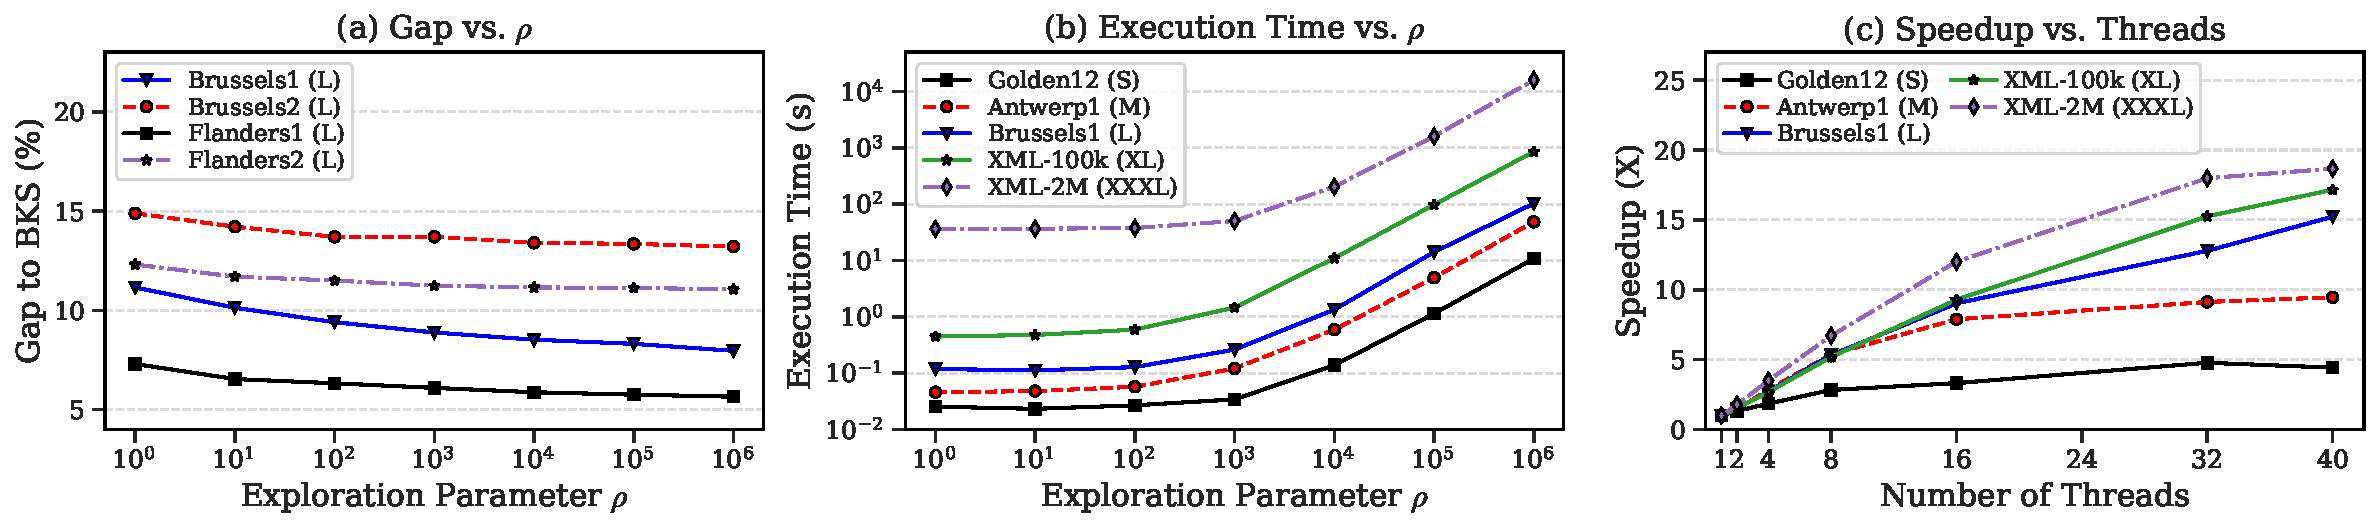
\includegraphics[
    width=\linewidth,
    keepaspectratio
]{sections/results/Parameter_sensitivity.pdf}
    \caption{(a--b) Impact of $\rho$ on solution quality and computational time; (c) Scalability with increasing thread count}
    \label{fig:unified_performance}
\end{figure*}

% ------------------------------------

\begin{figure*}[t]
    \centering
    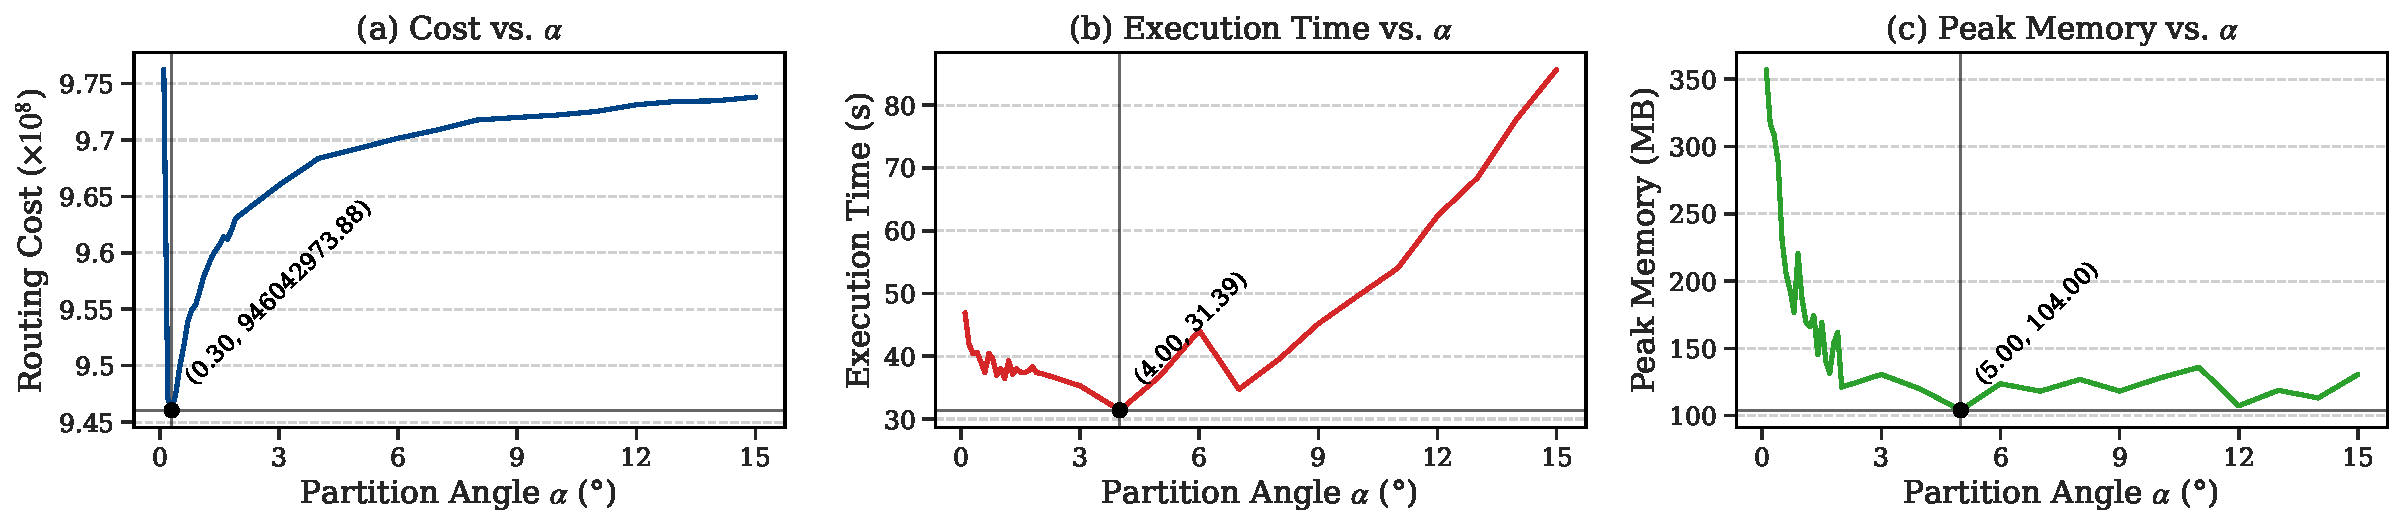
\includegraphics[
    width=\linewidth,
    keepaspectratio
]{sections/results/alpha/XML500000_1173_01_metrics.pdf}
    \caption{Effect of $\alpha$ on cost, execution time, and peak memory}
    \label{fig:alpha_sweep_page1}
\end{figure*}

\textbf{Computational Speedup:} Fig.~\hyperref[fig:parMDS_comparison_grid1]{\ref*{fig:parMDS_comparison_grid1}(a)} shows that BP-MDS achieves consistent execution speedups across all instances, ranging from $5\times$--$10\times$ for S and increasing to $20\times$--$60\times$ for M and L, indicating improved scaling with problem size. The observed speedups stem from massive parallelism and optimized data structures in BP-MDS, absent in ParMDS. 

\textbf{Memory Efficiency:} Fig.~\hyperref[fig:parMDS_comparison_grid1]{\ref*{fig:parMDS_comparison_grid1}(b)} shows that BP-MDS achieves substantial memory savings. While footprints are comparable for small instances, BP-MDS reduces memory usage by $\sim\!100\times$ on M and over $1000\times$ on L instances, enabling scalability to million-node graphs where ParMDS encounters out-of-memory failures. 

\textbf{Solution Quality:} Fig.~\hyperref[fig:parMDS_comparison_grid1]{\ref*{fig:parMDS_comparison_grid1}(c)} shows that BP-MDS consistently reduces the optimality gap across all benchmarks. Gap reductions exceed $10\%$ on S instances and are consistently observed across all evaluated instance sizes, indicating that scalability does not come at the expense of solution quality.

\subsubsection{Comparison Against HGS-CVRP}


\textsc{HGS-CVRP}~\cite{vidal2022hybrid} is a state-of-the-art CVRP solver that delivers high-quality solutions for small instances. Rather than comparing only final solution costs, we perform a time-to-quality analysis. For M and L instances, we measure the time required for HGS-CVRP to match or surpass the solution quality achieved by BP-MDS. For S instances, we report the time to convergence after 20{,}000 iterations. To ensure a fair algorithmic comparison with the single-threaded HGS-CVRP solver, we evaluate BP-MDS under both single-threaded (1T) and 40-threaded (40T) configurations (Table~\ref{tab:bpmds_vs_hgs_time}). For small instances, HGS-CVRP requires between 53 and 108 seconds to converge, whereas BP-MDS executes in under 1 second on a single thread and around $0.1$ seconds using 40 threads. The performance improvement is most pronounced on massive topologies, as observed for \texttt{Flanders1}: BP-MDS generates a high-quality routing plan (5.92\% gap) in just 30.78 seconds with 1 thread and 1.34 seconds with 40 threads, whereas HGS-CVRP takes nearly an hour to achieve the same solution quality. Ultimately, while HGS-CVRP is designed for exhaustive offline optimization to obtain highly optimal solutions, BP-MDS achieves functional routing solutions roughly $90\times$ to $100\times$ faster on a single thread and $350\times$ to $2370\times$ faster using 40 threads, making it well suited for real-time dynamic routing applications across small to massive instances.

\begin{table}[htbp]
\caption{Time-to-quality comparison: BP-MDS vs. HGS-CVRP}
\centering
\small
\setlength{\tabcolsep}{0pt}
\begin{tabular*}{\columnwidth}{@{\extracolsep{\fill}} l c r r r r r r @{}}
\toprule
& & \multicolumn{3}{c}{\textbf{HGS-CVRP}} & \multicolumn{3}{c}{\textbf{BP-MDS (at optimal $\alpha$)}} \\
\cmidrule(lr){3-5} \cmidrule(l){6-8}
\textbf{Instance} & \textbf{Size} & \textbf{Iter.} & \textbf{Time (s)} & \textbf{Gap (\%)} & \textbf{1T (s)} & \textbf{40T (s)} & \textbf{Gap (\%)} \\
\midrule
Golden\_17 & S & 20,000 &   53.80  & 0    &  0.60 & 0.07 & 7.76 \\
Golden\_18 & S & 20,000 &  108.30  & 0    &  0.81 & 0.12 & 4.97 \\
\midrule
Leuven1    & M &      0 &   61.06  & 5.19 &  5.20 & 0.49 & 7.64 \\
Antwerp1   & M &      0 &  185.96  & 5.38 & 10.06 & 0.53 & 7.29 \\
\midrule
Brussels1  & L &     38 & 1562.03  & 8.42 & 23.59 & 1.01 & 8.56 \\
Flanders1  & L &    138 & 3181.58  & 5.62 & 30.78 & 1.34 & 5.92 \\
\bottomrule
\multicolumn{8}{l}{\footnotesize 1T and 40T denote 1 and 40 threads, respectively}
\end{tabular*}
\label{tab:bpmds_vs_hgs_time}
\end{table}

% \begin{table}[htbp]
% \centering
% \setlength{\tabcolsep}{0pt} 
% \begin{tabular*}{\columnwidth}{@{\extracolsep{\fill}} l c r r r r r @{}}
% \toprule
% & & \multicolumn{3}{c}{\textbf{HGS-CVRP}} & \multicolumn{2}{c}{\textbf{BP-MDS}} \\
% \cmidrule(lr){3-5} \cmidrule(l){6-7}
% \textbf{Instance} & \textbf{Size} & \textbf{Iter.} & \textbf{Time (s)} & \textbf{Gap (\%)} & \textbf{Time (s)} & \textbf{Gap (\%)} \\
% \midrule
% Golden\_17 & S & 20,000 &  53.80  & 0 & 0.07 & 4.97  \\
% Golden\_18 & S & 20,000 &  108.30 & 0 & 0.12 & 7.76  \\
% \midrule
% Leuven1    & M &      0 &   61.06 &  5.19 & 0.49 &  7.64 \\
% Antwerp1   & M &      0 &  185.96 &  5.38 & 0.53 &  7.29 \\
% \midrule
% Brussels1  & L &     38 & 1562.03 &  8.42 & 1.01 &  8.56 \\
% Flanders1  & L &    138 & 3181.58 &  5.62 & 1.34 &  5.92 \\
% \bottomrule
% \end{tabular*}
% \caption{Time-to-Quality Comparison: BPMDS vs HGS-CVRP}
% \label{tab:bpmds_vs_hgs_time}
% \end{table}





\subsection{Scalability Study of BP-MDS}
\label{sec:strong_scaling}

\textbf{Execution time and memory scalability:} Figs.~\hyperref[fig:scalability_grid]{\ref*{fig:scalability_grid}(a,b)} show that both execution time and memory consumption increase steadily with problem size. The near-linear growth in execution time demonstrates that BP-MDS scales efficiently to XXXL instances, while the consistent memory trend confirms that bucket partitioning effectively bounds memory overhead.


\textbf{Parallel Scalability:} We evaluate scalability by varying the number of threads from 1 to 40 (Fig.~\hyperref[fig:unified_performance]{\ref*{fig:unified_performance}(c)}). To improve cache locality and avoid thread migration overhead, we enforce thread affinity via \texttt{OMP\_PLACES=cores} and \path{OMP_PROC_BIND=close}. For S and M instances, speedup saturates early and stabilizes well before 40 threads. In these cases, the limited number of angular buckets leads to short MST computations, making OpenMP overhead and thread management dominate useful computation. \REM{As a result, available cores cannot be fully utilized, yielding diminishing returns at higher thread counts.} In contrast, BP-MDS scales efficiently on L--XXXL instances, achieving up to $19\times$ speedup on 40 threads through the high degree of task parallelism provided by thousands of independent angular buckets.

% ------------------------------------
% --- FIGURE: ABLATION STUDY (MINHEAP & DFS PATTERNS) ---
\begin{figure*}[t]
    \centering
    % 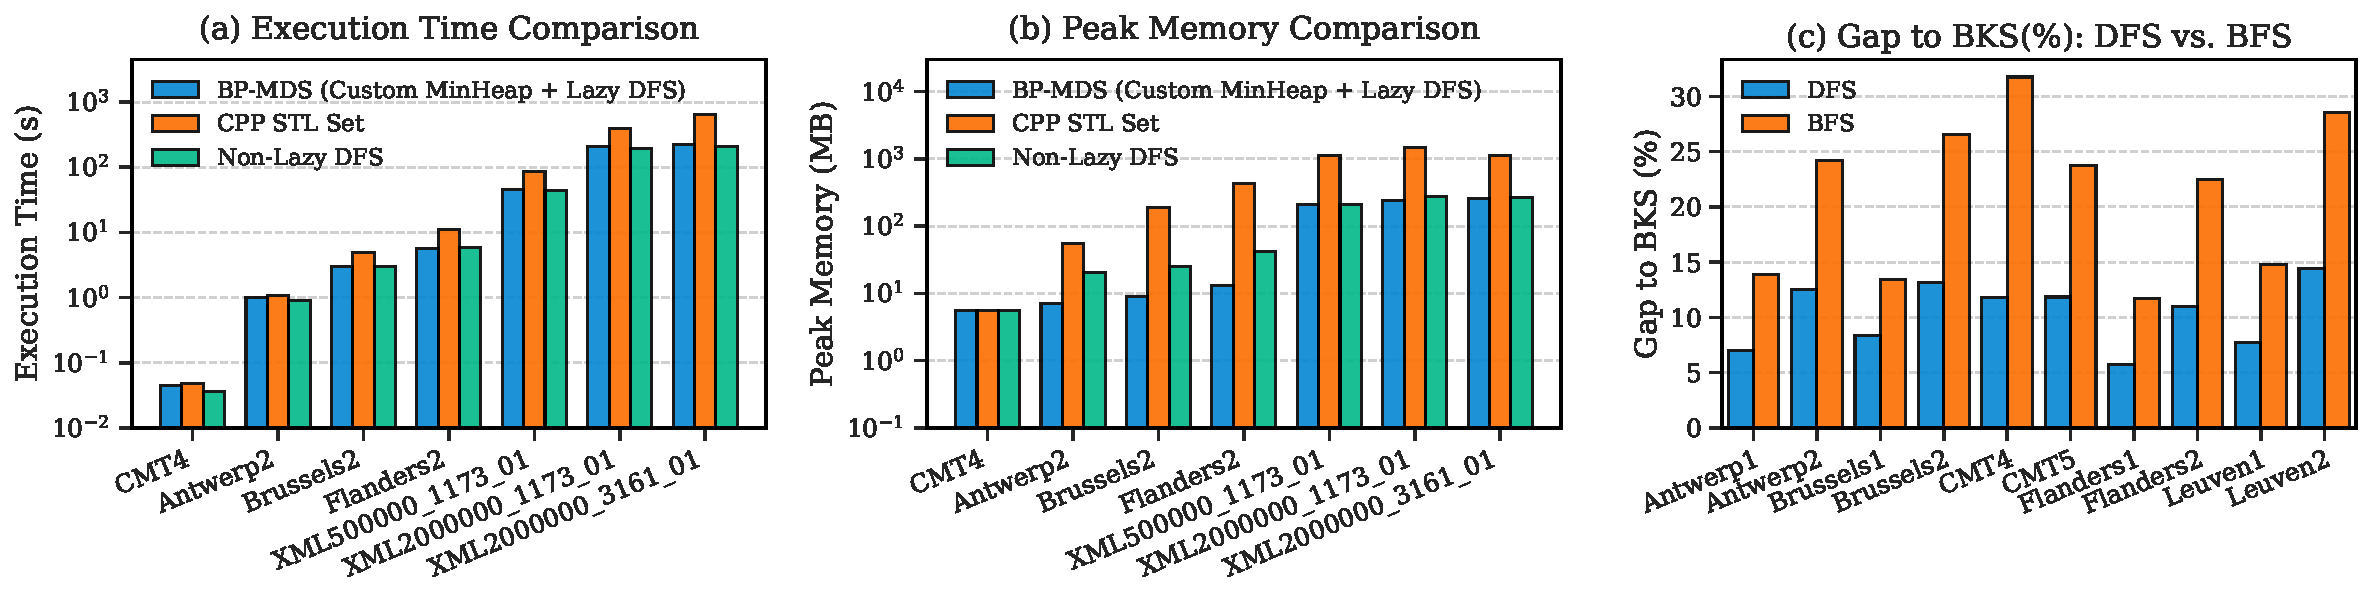
\includegraphics[width=\linewidth]{sections/results/Combined_Ablation_Analysis_Patterns.pdf}

    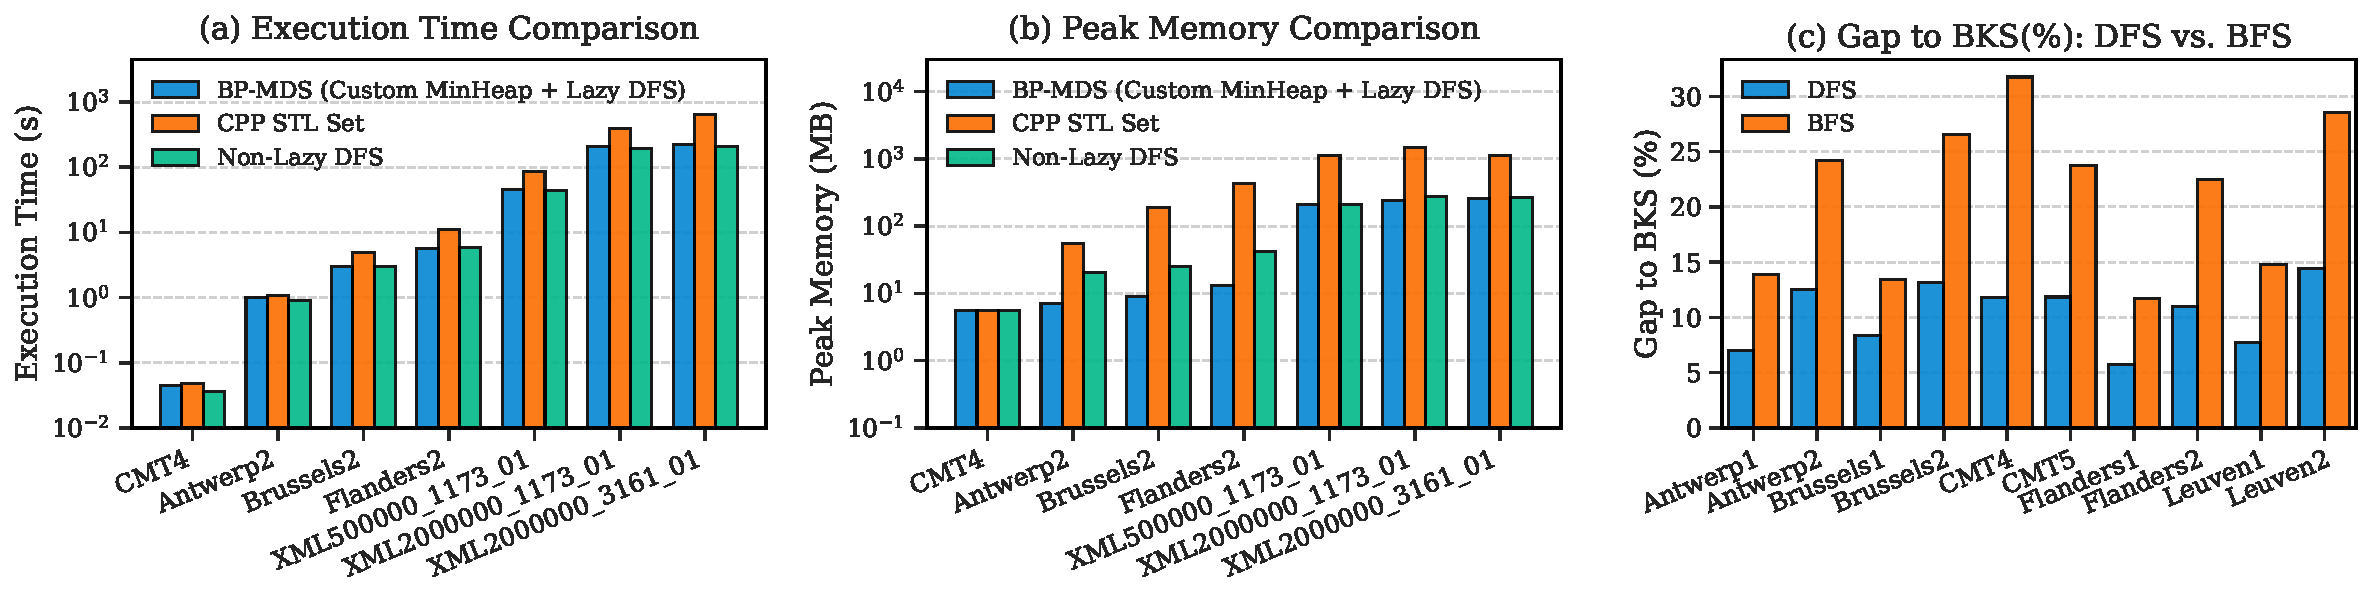
\includegraphics[
    width=\linewidth,
    keepaspectratio
]{sections/results/Combined_Ablation_Analysis_Patterns.pdf}
    \caption{BP-MDS ablation study: Benefits of the custom MinHeap and Lazy DFS, and DFS vs. BFS}
    \label{fig:ablation_analysis}
\end{figure*}



\subsection{Parameter Sensitivity Analysis}
\label{sec:scalability}

\subsubsection{\textbf{Angular Partition Parameter $\alpha$:}} Fig.~\ref{fig:alpha_sweep_page1} illustrates the effect of varying $\alpha$ on solution quality, execution time, and memory consumption. $\alpha$ significantly influences both performance and cost: smaller values of $\alpha$ increase the number of buckets, enabling higher parallelism but also altering solution structure. We select $\alpha$ corresponding to the minimum cost as the empirically best value and refer to it as the optimal $\alpha$ for a given instance size. Fig.~\hyperref[fig:scalability_grid]{\ref*{fig:scalability_grid}(c)} shows that the angular partition parameter $\alpha$ decreases with increasing problem size. This inverse relationship reflects the need for finer bucket partitioning in larger instances, where customer distributions become increasingly structured and exhibit a “flower-like” geometry (Figs.~\ref{fig:BKS_Brussels} and~\ref{fig:2-d-partition}). This enables finer angular buckets to group spatially correlated customers, improving route coherence. 

\textbf{Estimating the Optimal Partition Angle:} The cost-effective $\alpha$ depends on graph scale and spatial density, making manual tuning an additional step in the execution of BP-MDS. To remove this dependency, we propose a simple predictive model that estimates a baseline $\alpha$ directly from graph properties. We use a log-log linear regression with two features: graph dimension ($N$) and total demand-to-capacity ratio ($TD/Q$). Since spatial parameters often follow power-law behavior in routing problems \cite{daganzo1984distance}, we perform regression in logarithmic space, generating a linearized model, a standard approach for modeling multiplicative relationships \cite{hastie2009elements}: $\ln(\alpha) = \ln(k) + c_1 \ln(N) + c_2 \ln\left(\frac{TD}{Q}\right)$. The model is trained on 149 instances ($N > 1000$) with an 80:20 split. In the original scale, it achieves $R^2=0.8376$ (train) and $0.9311$ (test). The learned relation is $\alpha = 949.2975 \cdot N^{-0.1016} \cdot \left(\frac{TD}{Q}\right)^{-0.5509}$, with a test MAE of $3.17^\circ$. \REM{While effective for initialization, incorporating topological features such as route size and depot position may further improve accuracy.}


\subsubsection{\textbf{Exploration Parameter $\rho$}} Increasing $\rho$ reduces the optimality gap (Fig.~\hyperref[fig:unified_performance]{\ref*{fig:unified_performance}(a)}), with the largest gains in the early regime ($\rho \le 10^3$) where randomized DFS quickly identifies high-quality edge combinations. Beyond this, improvements saturate as the local search space within each bucket is exhausted. While low $\rho$ yields higher gaps due to limited exploration, increasing $\rho$ stabilizes solution quality, indicating that BP-MDS avoids poor local optima despite partitioning. However, since the computational effort increases with $\rho$, the execution time also rises accordingly (Fig.~\hyperref[fig:unified_performance]{\ref*{fig:unified_performance}(b)}). Balancing quality and cost, $\rho = 10^4$ emerges as a sweet spot, achieving over $95\%$ of the attainable improvement with modest runtime. \REM{Further increases incur significant overhead with negligible gains.}

% \subsection{Implementation Ablation Study}
\subsection{Ablation Study}
\label{sec:ablation_study} 

\begin{figure*}
    \centering
    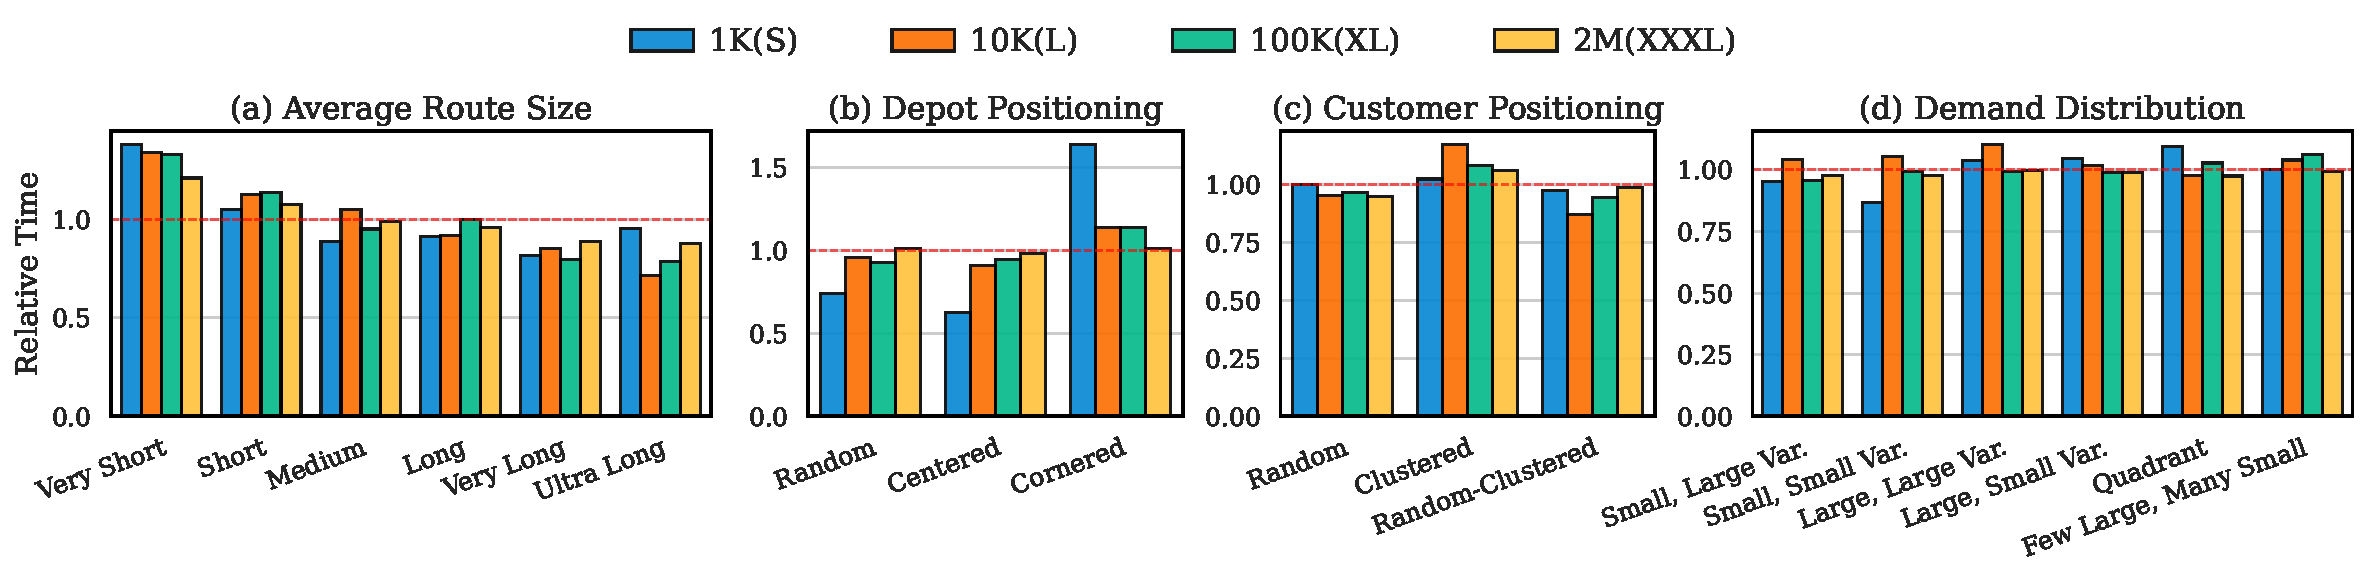
\includegraphics[width=0.94\linewidth]{sections/results/time_plot.pdf}
    
    {\footnotesize Relative time $= T_{g,c}/\bar{T}_g$, where $\bar{T}_g=\frac{1}{|C_g|}\sum_{c\in C_g} T_{g,c}$ is the mean execution time over all instances in category set $C_g$ for graph size $g$}
    \caption{Impact of input characteristics on execution time (at the optimal $\alpha$)}
    \label{fig:characteristics}
\end{figure*}

\begin{figure*}[h]
    \centering
    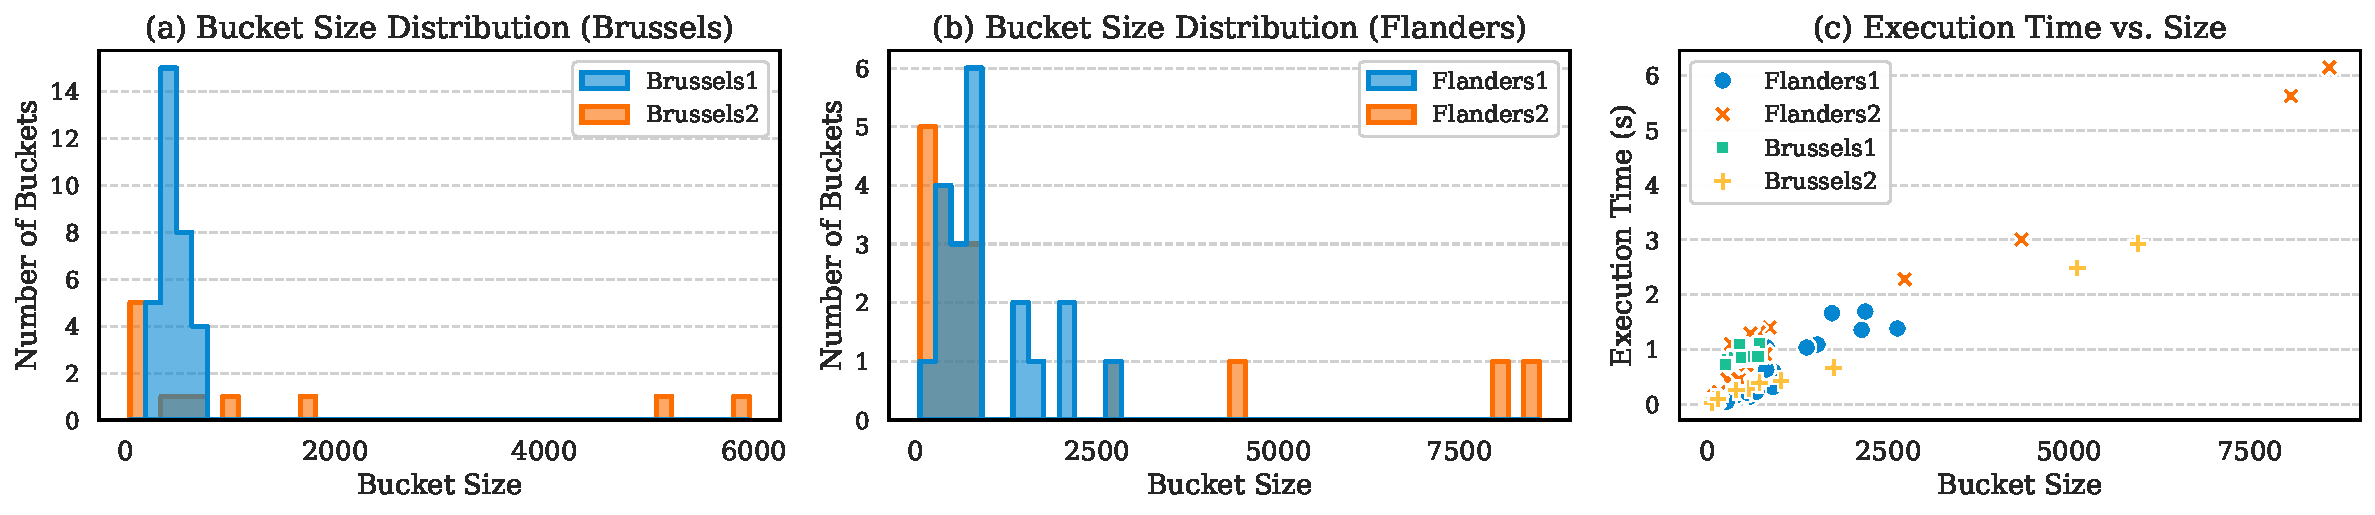
\includegraphics[
    width=\linewidth,
    keepaspectratio
]{sections/results/Bucket_Analysis.pdf}
    \caption{Analysis of centered vs. cornered depots (at the optimal $\alpha$)}
    \label{fig:bucket_analysis}
\end{figure*}

We evaluate three key design choices (Fig.~\ref{fig:ablation_analysis}): a custom MinHeap for Prim's MST, lazy vs. eager DFS, and DFS vs. BFS.


\textbf{Custom MinHeap vs. C++ \texttt{std::set}:} After bucket construction, each thread builds an MST using Prim's algorithm. Our custom \texttt{Min\_Heap} achieves up to a $2.9\times$ speedup (Fig.~\hyperref[fig:ablation_analysis]{\ref*{fig:ablation_analysis}(a)}) by supporting in-place \texttt{DecreaseKey} operations, whereas \texttt{std::set} inserts redundant entries for updated distances, increasing logarithmic overhead. This also substantially reduces memory usage (Fig.~\hyperref[fig:ablation_analysis]{\ref*{fig:ablation_analysis}(b)}): on XXXL instances, \texttt{std::set} uses up to 1.56\,GB due to stale entries, while the custom heap stores one entry per vertex, requiring only 279\,MB.

\textbf{Lazy vs. Eager DFS Traversal:} To generate multiple randomized routes, the MST adjacency list is shuffled before each DFS traversal. \textit{Lazy DFS} copies and shuffles neighbors on demand when a vertex is visited, whereas \textit{Eager DFS} precomputes a deep copy of the entire MST before traversal. Although Eager DFS is marginally faster on large-scale graphs (Fig.~\hyperref[fig:ablation_analysis]{\ref*{fig:ablation_analysis}(a)}), it increases peak memory usage by up to $2.7\times$ (Fig.~\hyperref[fig:ablation_analysis]{\ref*{fig:ablation_analysis}(b)}). In contrast, Lazy DFS bounds per-thread memory consumption while maintaining comparable runtime, making it the preferred strategy for BP-MDS.


\textbf{Why DFS?:} BP-MDS constructs routes by sequentially partitioning the MST traversal order into capacity-feasible routes. By following contiguous root-to-leaf paths, DFS preserves MST connectivity, increasing the likelihood that adjacent vertices in the MST remain within the same route. In contrast, BFS alternates between sibling vertices at the same level, fragmenting MST edges across routes. Consequently, DFS produces lower routing costs than BFS (Fig.~\hyperref[fig:ablation_analysis]{\ref*{fig:ablation_analysis}(c)}). On Flanders (1-2), BFS doubles the optimality gap of DFS.

% Flanders1: BFS\_gap=11.72\%, DFS\_gap=5.78\%, Flanders2: BFS\_gap=22.51\%, DFS\_gap=10.99\%

\subsection{Impact of Input Characteristics}
\label{sec:topology_impact}

% Notes for relative time measurement:
% Times are normalized independently within each graph size category (1K, 10K, 100K, 2M) by dividing by the mean execution time of that scale. The red dashed line ($y = 1.0$) denotes the average computational cost for a graph of that size, highlighting which structural traits inflate or reduce execution overhead.
% For example in subplot (a), for 1K S instances, the mean of all the 6 blue bars is taken and for each bar the time there is divided by this mean. This is done for all S, L, XXL, XXXL seperately

% 

BP-MDS is evaluated on diverse input characteristics (Fig.~\ref{fig:characteristics}) generated using the CVRPLIB input generator. Execution time decreases as the average route size increases, since longer routes reduce the overhead of repeatedly switching between buckets in a parallel setting (Fig.~\hyperref[fig:characteristics]{\ref*{fig:characteristics}(a)}). For the 2M-node instances, increasing the average route size from \emph{Very Short} to \emph{Ultra Long} reduces execution time from 204.04\,s to 151.68\,s. Cornered-depot instances generally require higher execution time than centered or randomly positioned depots (Fig.~\hyperref[fig:characteristics]{\ref*{fig:characteristics}(b)}). This is because cornered depots produce unbalanced bucket sizes, increasing the workload of the largest bucket. On 1K (S) graphs, the cornered depot incurs a $2.47\times$ higher execution time than the centered depot. This behavior is evident in Fig.~\hyperref[fig:bucket_analysis]{\ref*{fig:bucket_analysis}(a,b)}, where \texttt{Brussels2} and \texttt{Flanders2} (cornered depots) exhibit significantly larger buckets than \texttt{Brussels1} and \texttt{Flanders1} (centered depots) (spatial differences are visualized in Fig.~\ref{fig:BKS_Brussels}). Execution time strictly increases with the maximum bucket size (Fig.~\hyperref[fig:bucket_analysis]{\ref*{fig:bucket_analysis}(c)}), confirming that the largest bucket dominates the overall runtime. \REM{In contrast, customer positioning (Fig.~\hyperref[fig:characteristics]{\ref*{fig:characteristics}(c)}) and demand distribution (Fig.~\hyperref[fig:characteristics]{\ref*{fig:characteristics}(d)}) have minimal impact on execution time.}

% {\color{magenta} Demand Distribution among customers. Type 1 assigns a unitary demand of exactly $1$ to all customers, while Types 2 through 5 sample uniformly from fixed intervals: $[1, 10]$ (small, large variance), $[5, 10]$ (small, small variance), $[1, 100]$ (large, large variance), and $[50, 100]$ (large, small variance). For Quadrant, Customers in "even quadrants" (bottom-left where $x,y < 5000$, or top-right where $x,y \ge 5000$) get large demands sampled uniformly from $[51, 100]$.  Customers in the other two quadrants get smaller demands sampled from $[1, 50]$. A calculated proportion of customers ($\frac{n}{r} \times 1.5$, where $r$ is target route size) receive large demands uniformly sampled from $[50, 100]$.  All remaining customers receive small demands sampled from $[1, 10]$. 
% Average Route Size (avgRouteSize) controls the expected number of customers served per vehicle by uniformly sampling a target continuous value $r$(route size) from one of six category intervals: Very short $[3, 5]$, Short $[5, 8]$, Medium $[8, 12]$, Long $[12, 16]$, Very long $[16, 25]$, and Ultra long $[25, 50]$. 
% Depot Positioning establishes the starting hub location on a $10{,}000 \times 10{,}000$ 2D Euclidean grid according to three simple placement strategies. Type 1 (Random) places the depot uniformly at random anywhere within the $[0, 10000]$ coordinate range. Type 2 (Centered) fixes the depot exactly at the midpoint of the grid at coordinates $(5000, 5000)$. Type 3 (Cornered) fixes the depot at the bottom-left origin point $(0, 0)$.  
% Customer Positioning (custPos) distributes the $n$ customer coordinates across the same $10{,}000 \times 10{,}000$ Euclidean grid using three distinct spatial patterns. Type 1 (Random) generates all customer coordinates uniformly at random across the entire grid. Type 2 (Clustered) generates between 2 to 6 random seed centers and places customers around them using an Accept-Reject method. Type 3 (Random-Clustered) is a 50/50 hybrid model where half of the customers ($n/2$) are generated uniformly at random and the remaining half are generated around seed centers using the exponential decay clustering method.}

%  The below two paras are related to: Impact of graph topology on alpha. This is removed because of lack of space. 
% Fig.~\hyperref[fig:characteristics]{\ref*{fig:characteristics}(a)} shows that $\alpha$ increases with average route size, since larger routes require a wider angular sweep to accumulate sufficient customers for feasible vehicle capacity. Fig.~\hyperref[fig:characteristics]{\ref*{fig:characteristics}(b)} shows that a centered depot yields higher $\alpha$ than cornered or random placements, as central positioning spreads customers over a full $360^\circ$ range, requiring wider partitions to capture enough nodes per bucket. Fig.~\hyperref[fig:characteristics]{\ref*{fig:characteristics}(c)} shows that clustered customer distributions also increase $\alpha$, as overly narrow partitions fragment spatial clusters and break short-distance route coherence.

% Across all cases, graph scale dominates these effects: as the number of nodes increases, sensitivity to topology diminishes and $\alpha$ consistently converges to smaller angular values. This is because higher node density reduces the need for wide partitions, allowing efficient routing within narrow angular regions. Overall, BP-MDS adapts to topology at small scales but becomes scale-dominated, where dense graphs enforce uniform, highly fine-grained partitioning without loss of routing quality.


